\chapter{\textbf{Metodología}}\label{ch:metodos}

La herramienta de trabajo principal que vamos a utilizar a lo largo de nuestro estudio es el software \textbf{\textit{CST Studio Suite 2010}}, el cual permite realizar simulaciones de antenas con sus resultados de ganancia, directividad, campos y diversas medidas. Entraremos en detalle en este capítulo en el principal uso que le vamos a dar: diseñar y simular antenas microstrip.


\section{Introducción al software CST}

El software CST proviene de las siglas de \textit{Computer Simulation Technology} el cual es un programa que permite diseñar y simular aplicaciones para filtros, conectores, antenas, capacitores, inductancias, guías de onda y un sinfín de dispositivos que se pueden modelar~\cite{cst}.

\begin{figure}[!htb]
    \centering
    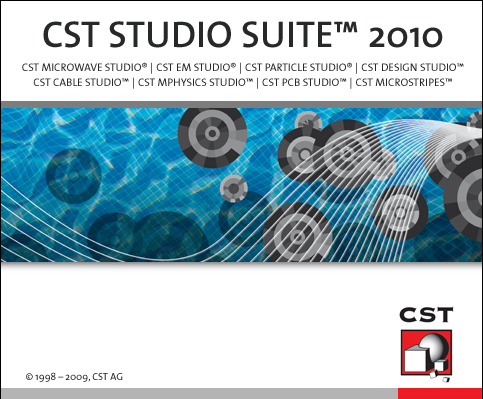
\includegraphics[scale=0.35]{./Metodologia/CST_Intro}
    \caption{Logo del programa CST Studio Suite 2010.}
    \label{fig:fig4.1}
\end{figure}

Una vez iniciado el programa tenemos la posibilidad de elegir el tipo de problema al que nos vamos a enfrentar, es decir, podemos elegir de qué manera va a ir encaminado nuestro proyecto, ya que si elegimos una opción u otra, las condiciones en las que trabajaremos serán muy distintas. Como podemos ver en la \textit{fig. \ref{fig:fig4.2}}, se nos presentan ocho opciones a elegir, desde un proyecto que engloba un estudio electromagnético, pasando por un estudio de partículas o incluso un estudio de conectores o de líneas microstrip.

\begin{figure}[!htb]
    \centering
    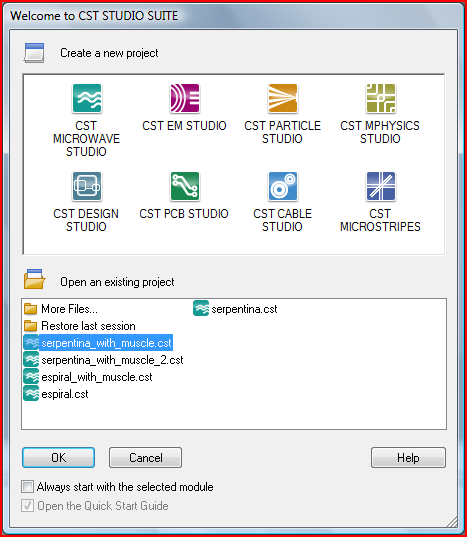
\includegraphics[scale=0.45]{./Metodologia/CST_Open_folder}
    \caption{Ventana introductoria del CST Studio Suite 2010.}
    \label{fig:fig4.2}
\end{figure}

En el marco en el que nos encontramos, de todas esas opciones la elegida por nosotros será \textbf{CST MICROWAVE STUDIO}, es decir, un proyecto en el que se diseñan y simulan dispositivos que trabajan a frecuencas de microondas, como los teléfonos móviles, dispositvos aeronáuticos o como en nuestro caso, antenas planas o de parche.

\subsection{Entorno de trabajo del software CST}\label{subsec:entorno-de-trabajo-del-software-cst}

Después de elegir el tipo de proyecto en el que nos vamos a embarcar, el programa nos presenta una interfaz como la que podemos ver en la \textit{fig. \ref{fig:fig4.3}} bastante clara e intuitiva. En la parte de arriba, tenemos todas las herramientas a nuestra disposición para diseñar, fijar parámetros de nuestra antena y simular según unas condiciones. En la parte de la izquierda se recogen en un árbol de directorios todos los elementos de nuestro diseño, desde componentes, pasando por los materiales utilizados hasta las propias simulaciones y resultados en último lugar. En la parte de abajo, tenemos las variables globales que se pueden definir como queramos para facilitar la tarea de asignar valores a las medidas del diseño en proceso. Y por último, en la parte central, tenemos la aparencia de nuestro diseño en un entorno tridimensional.

\begin{figure}[!htb]
    \centering
    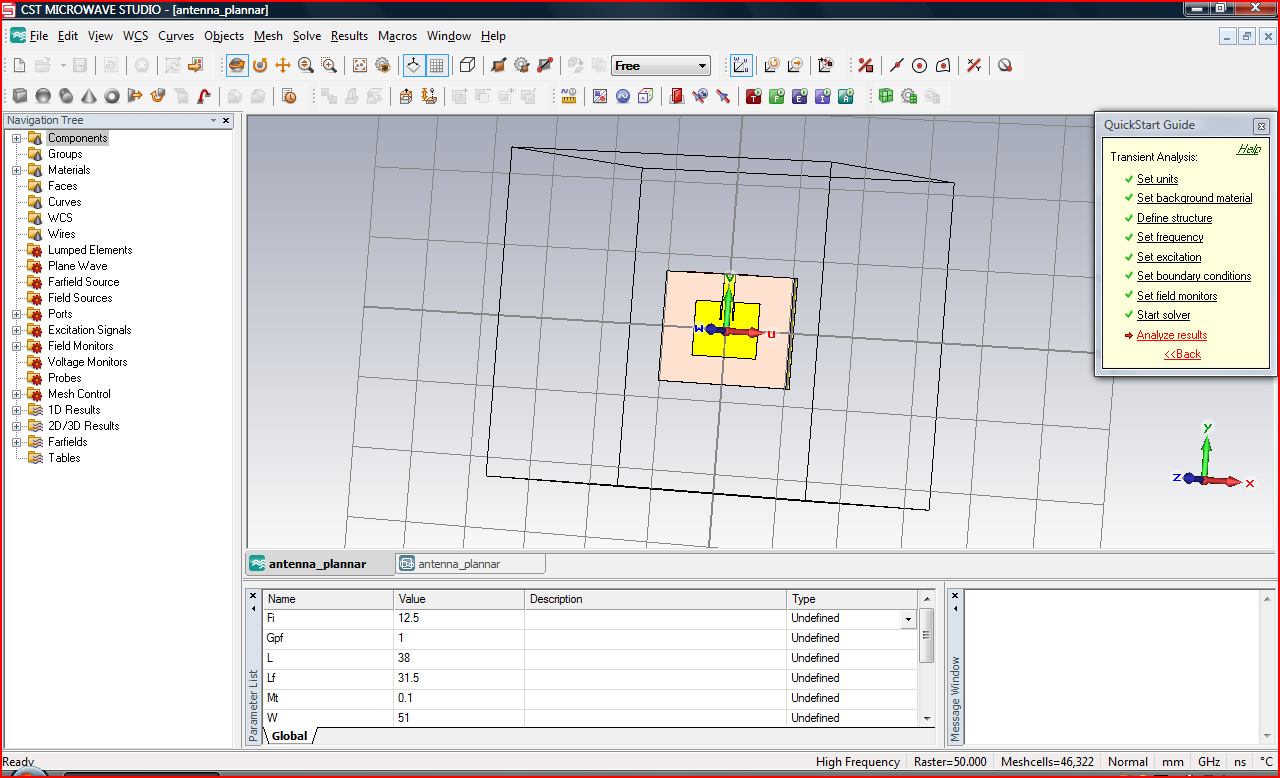
\includegraphics[scale=0.35]{./Metodologia/CST_first_window}
    \caption{Entorno de trabajo del CST Studio Suite 2010.}
    \label{fig:fig4.3}
\end{figure}

\subsection{Diseño antena ejemplo en CST}\label{subsec:diseno-antena-ejemplo-en-cst}

Lo primero que debemos hacer es dar información al CST sobre las medidas del diseño. Para ello tenemos la opción de crear variables globales con las que podremos dar forma a la antena, como por ejemplo, el largo y ancho, la altura del substrato o la longitud de la alimentación.

\clearpage

\begin{figure}[!htb]
    \centering
    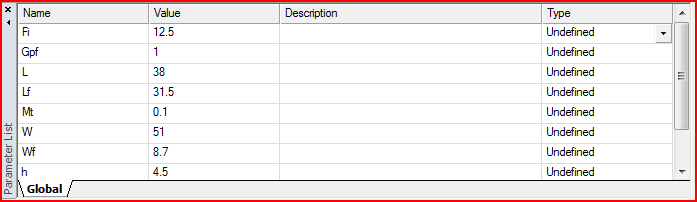
\includegraphics[scale=0.4]{./Metodologia/CST_global_parametres}
    \caption{Parámetros globales para el CST.}
    \label{fig:fig4.4}
\end{figure}

Una vez introducidas las variables globales, es el turno de construir nuestro diseño de la antena. En la barra de herramientas superior tenemos una serie de botones con distintas formas geométricas que se usan para crear las diferentes partes de la antena en tres dimensiones: cubos, hexaedros, conos, cilindros, toroides, etc. Existe incluso la opción de crear capas a partir de las ya creadas con la opción de \textit{extrude}.

\begin{figure}[!htb]
    \centering
    
\includegraphics[scale=0.7]{./Metodologia/CST_figures}
    \caption{Herramientas para la creación del dispositivo.}
    \label{fig:fig4.5}
\end{figure}

El paso siguiente a elegir el tipo de material de cada capa y sus correspondientes medidas, además de colocar adecuadamente la alimentación. Dicha alimentación puede ser un puerto discreto, simplemente unir conductor y dieléctrico o como una guía de onda, en la que tendremos que especificar las dimensiones de la misma. Dependiendo de dónde lo alimentemos y cómo, tendremos unos u otros resultados.

Cuando hayamos completado nuestro diseño procederemos a la etapa de simulación, la cual es clave en todo proyecto realizado en este software. Tenemos en primer lugar que elegir qué característica queremos medir: campo electromagnético, flujo magnético, corriente, etc. Esto se ve en \textit{fig. \ref{fig:fig4.6}}, que representa la ventana de \textit{monitor}.

\clearpage

\begin{figure}[!htb]
    \centering
    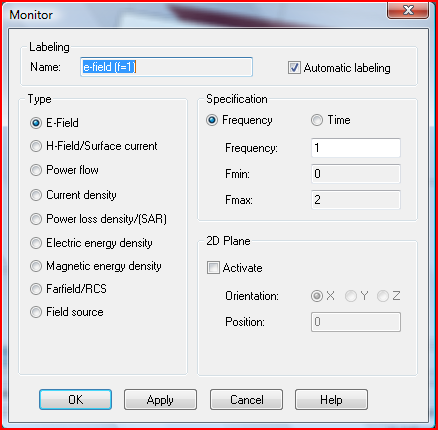
\includegraphics[scale=0.45]{./Metodologia/CST_monitor}
    \caption{Ventana \textit{monitor} con las distintas simulaciones y pruebas posibles.}
    \label{fig:fig4.6}
\end{figure}

El siguiente paso es ejectuar las tareas de simulación a través de la herramienta \textit{solver}. Elegimos de qué manera queremos que salgan los resultados, cuánta impedancia hay a la entrada, etc. y después tendremos los datos listos para revisarlos.

\begin{figure}[!htb]
    \centering
    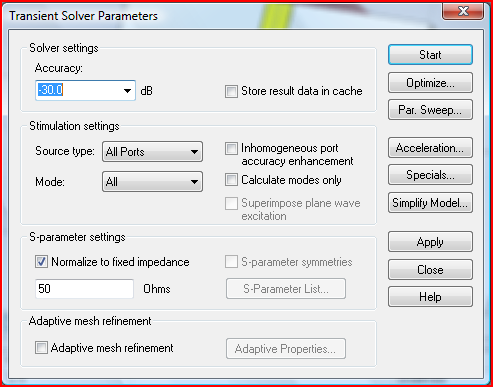
\includegraphics[scale=0.45]{./Metodologia/CST_solver}
    \caption{Ventana \textit{solver} con los parámetros disponibles para la simulación.}
    \label{fig:fig4.7}
\end{figure}

La última parte en la tarea del manejo del software CST será comprobar el diseño y las simulaciones conseguidas. En las siguientes imágenes podemos ver para un ejemplo concreto de antena microstrip, sus distintos resultados.

\clearpage

\begin{figure}[!htb]
    \centering
    \subfigure[]{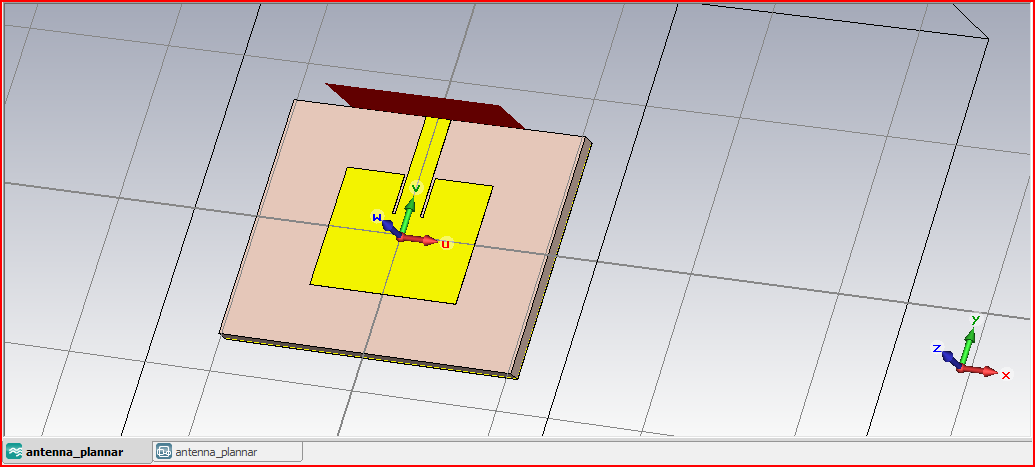
\includegraphics[scale=0.3]{./Metodologia/CST_antenna}}
    \subfigure[]{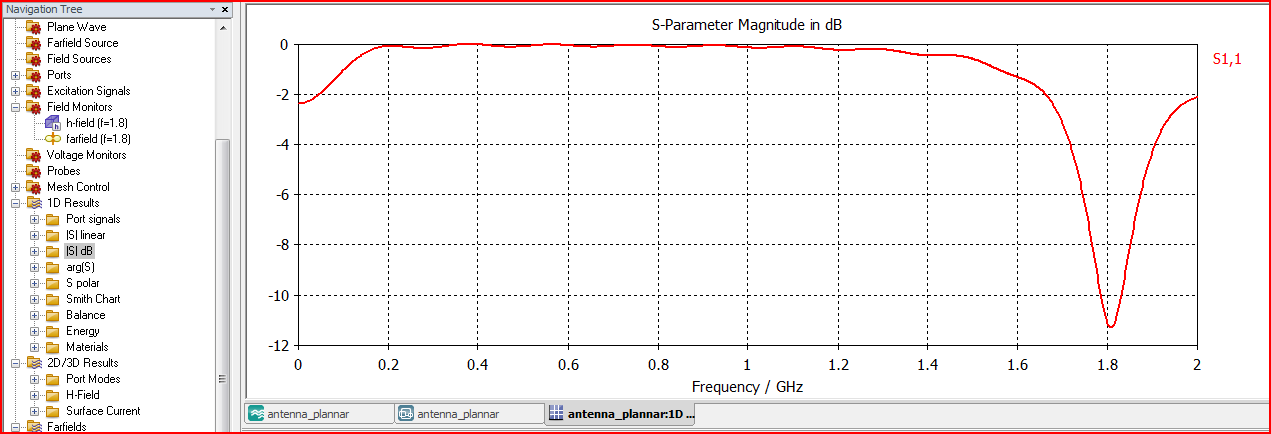
\includegraphics[scale=0.3]{./Metodologia/CST_dB}}
    \subfigure[]{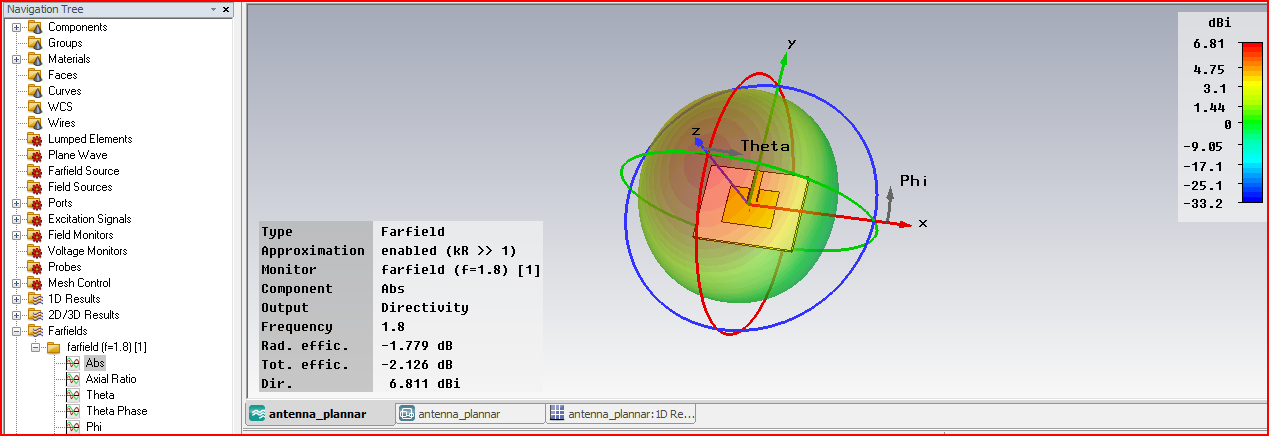
\includegraphics[scale=0.3]{./Metodologia/CST_farfield}}
    \caption{Imágenes tras el diseño y simulación de una antena ejemplo en el CST. En (a) un diseño final en 3D de una antena. En (b) gráfica del parámetro $S_{11}$. En (c) diagrama de radiación en 3D.}
    \label{fig:fig4.8}
\end{figure}

\clearpage


\section{Matlab como herramienta de apoyo}\label{sec:matlab-como-herramienta-de-apoyo}

El software \textbf{\textit{Matlab R2010b}} ha sido utilizado para crear las gráficas de los parámetros $S_{11}$ de las distintas simulaciones, además de las gráficas comparativas entre simulaciones del mismo parámetro.

Para ello, se ha obtenido del software CST los datos tabulados de cada simulación del parámetro $S_{11}$ por medio de un fichero de texto, el cual se ha metido como entrada un fichero \textbf{.m} de Matlab que se ha creado para este propósito.

\begin{figure}[!htb]
    \centering
    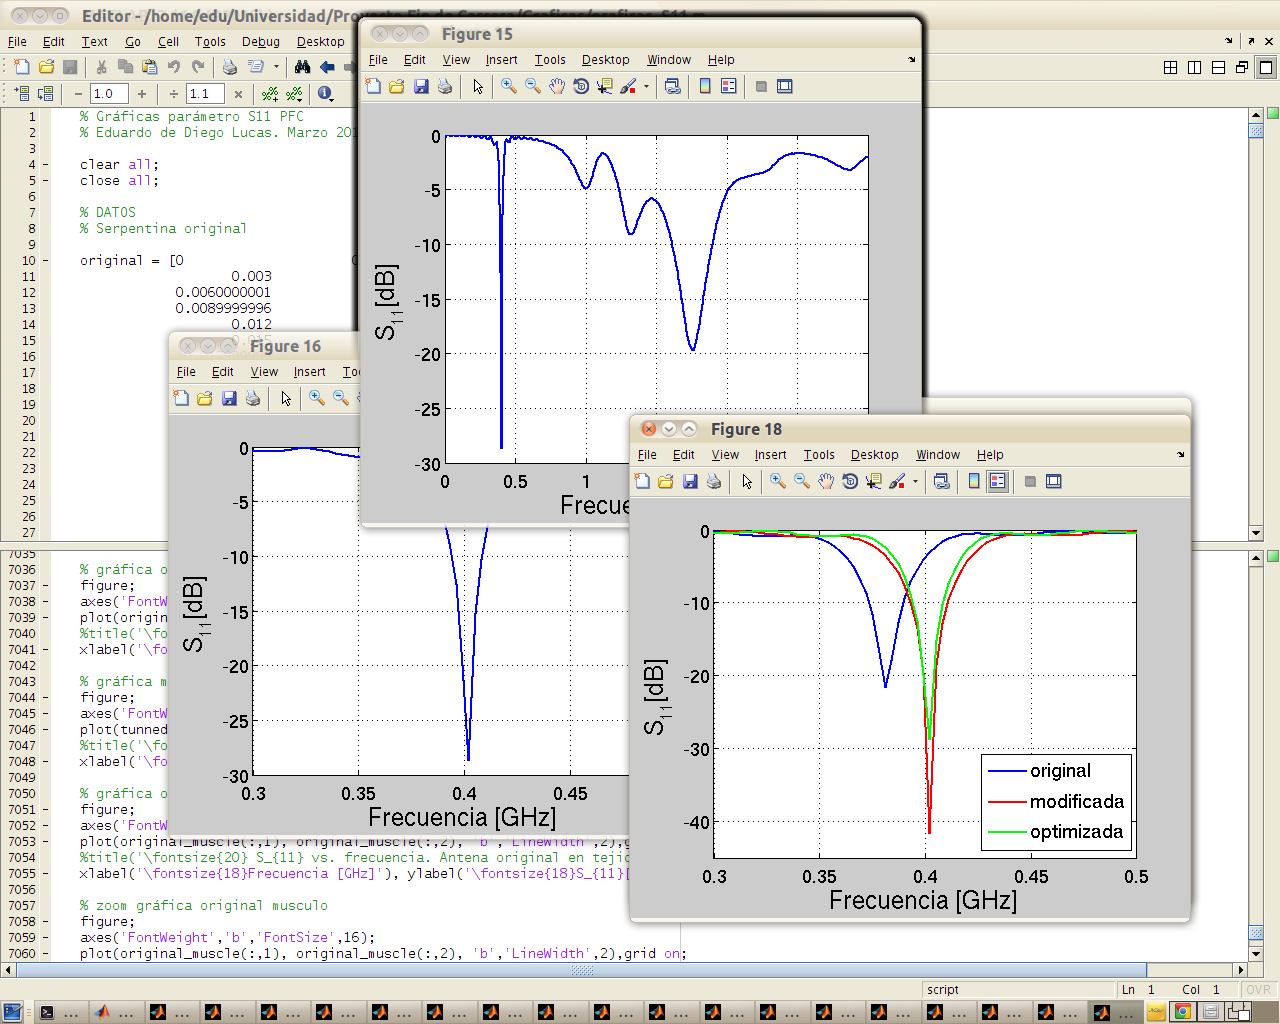
\includegraphics[scale=0.35]{./Metodologia/matlab2}
    \caption{Programa Matlab y su editor con distintas gráficas obtenidas del archivo creado.}
    \label{fig:fig4.9}
\end{figure}